% \chapter{Context and scientific contributions of this thesis}\label{chapter:contributions}
\chapter{Context and contributions of this thesis}\label{chapter:contributions}
\chaptermark{Scientific Contributions}
\newpage
\mbox{}
\newpage

The work in this thesis (\figref{fig:chapter2:overview}) began in late 2019, at the dawn of big data for structural biology with the first AlphaFold version \cite{senior_improved_2020}, but before its second version was able to predict most monomeric protein structures from structure at near-experimental resolutions \cite{jumper_highly_2021}. By then, two main voices summarised the state of structural biology: The first believed that the jump in performance for protein structure predictor was due to the change of approach and the inclusion of big data, but the expected evolution of the field would follow previously observed increments. The second believed that the final fold of a protein would soon be predicted from its sequence alone, and structural biology will have to move to different aspects of the protein folding problem \cite{alquraishi_alphafold_2018}, such as the protein \gls{foldingpath}, adoption of multiple \glspl{conformation}, and \gls{dynamics} \cite{powers_proteome_2021}. Just two years later, the latter was proven right when AlphaFold2 predicted protein structures with near-experimental accuracy. The work in this thesis contributes to the study of the remaining elements of the protein folding problem by providing metrics and software to quantify protein \glspl{conformationalensemble} and protein biophysical properties. It also contextualises AlphaFold's models in relation to the metrics here defined and in relation to previously-existing experimental and computational metrics of \gls{dynamics}.

\begin{figure}[tbh!]
    \centering
    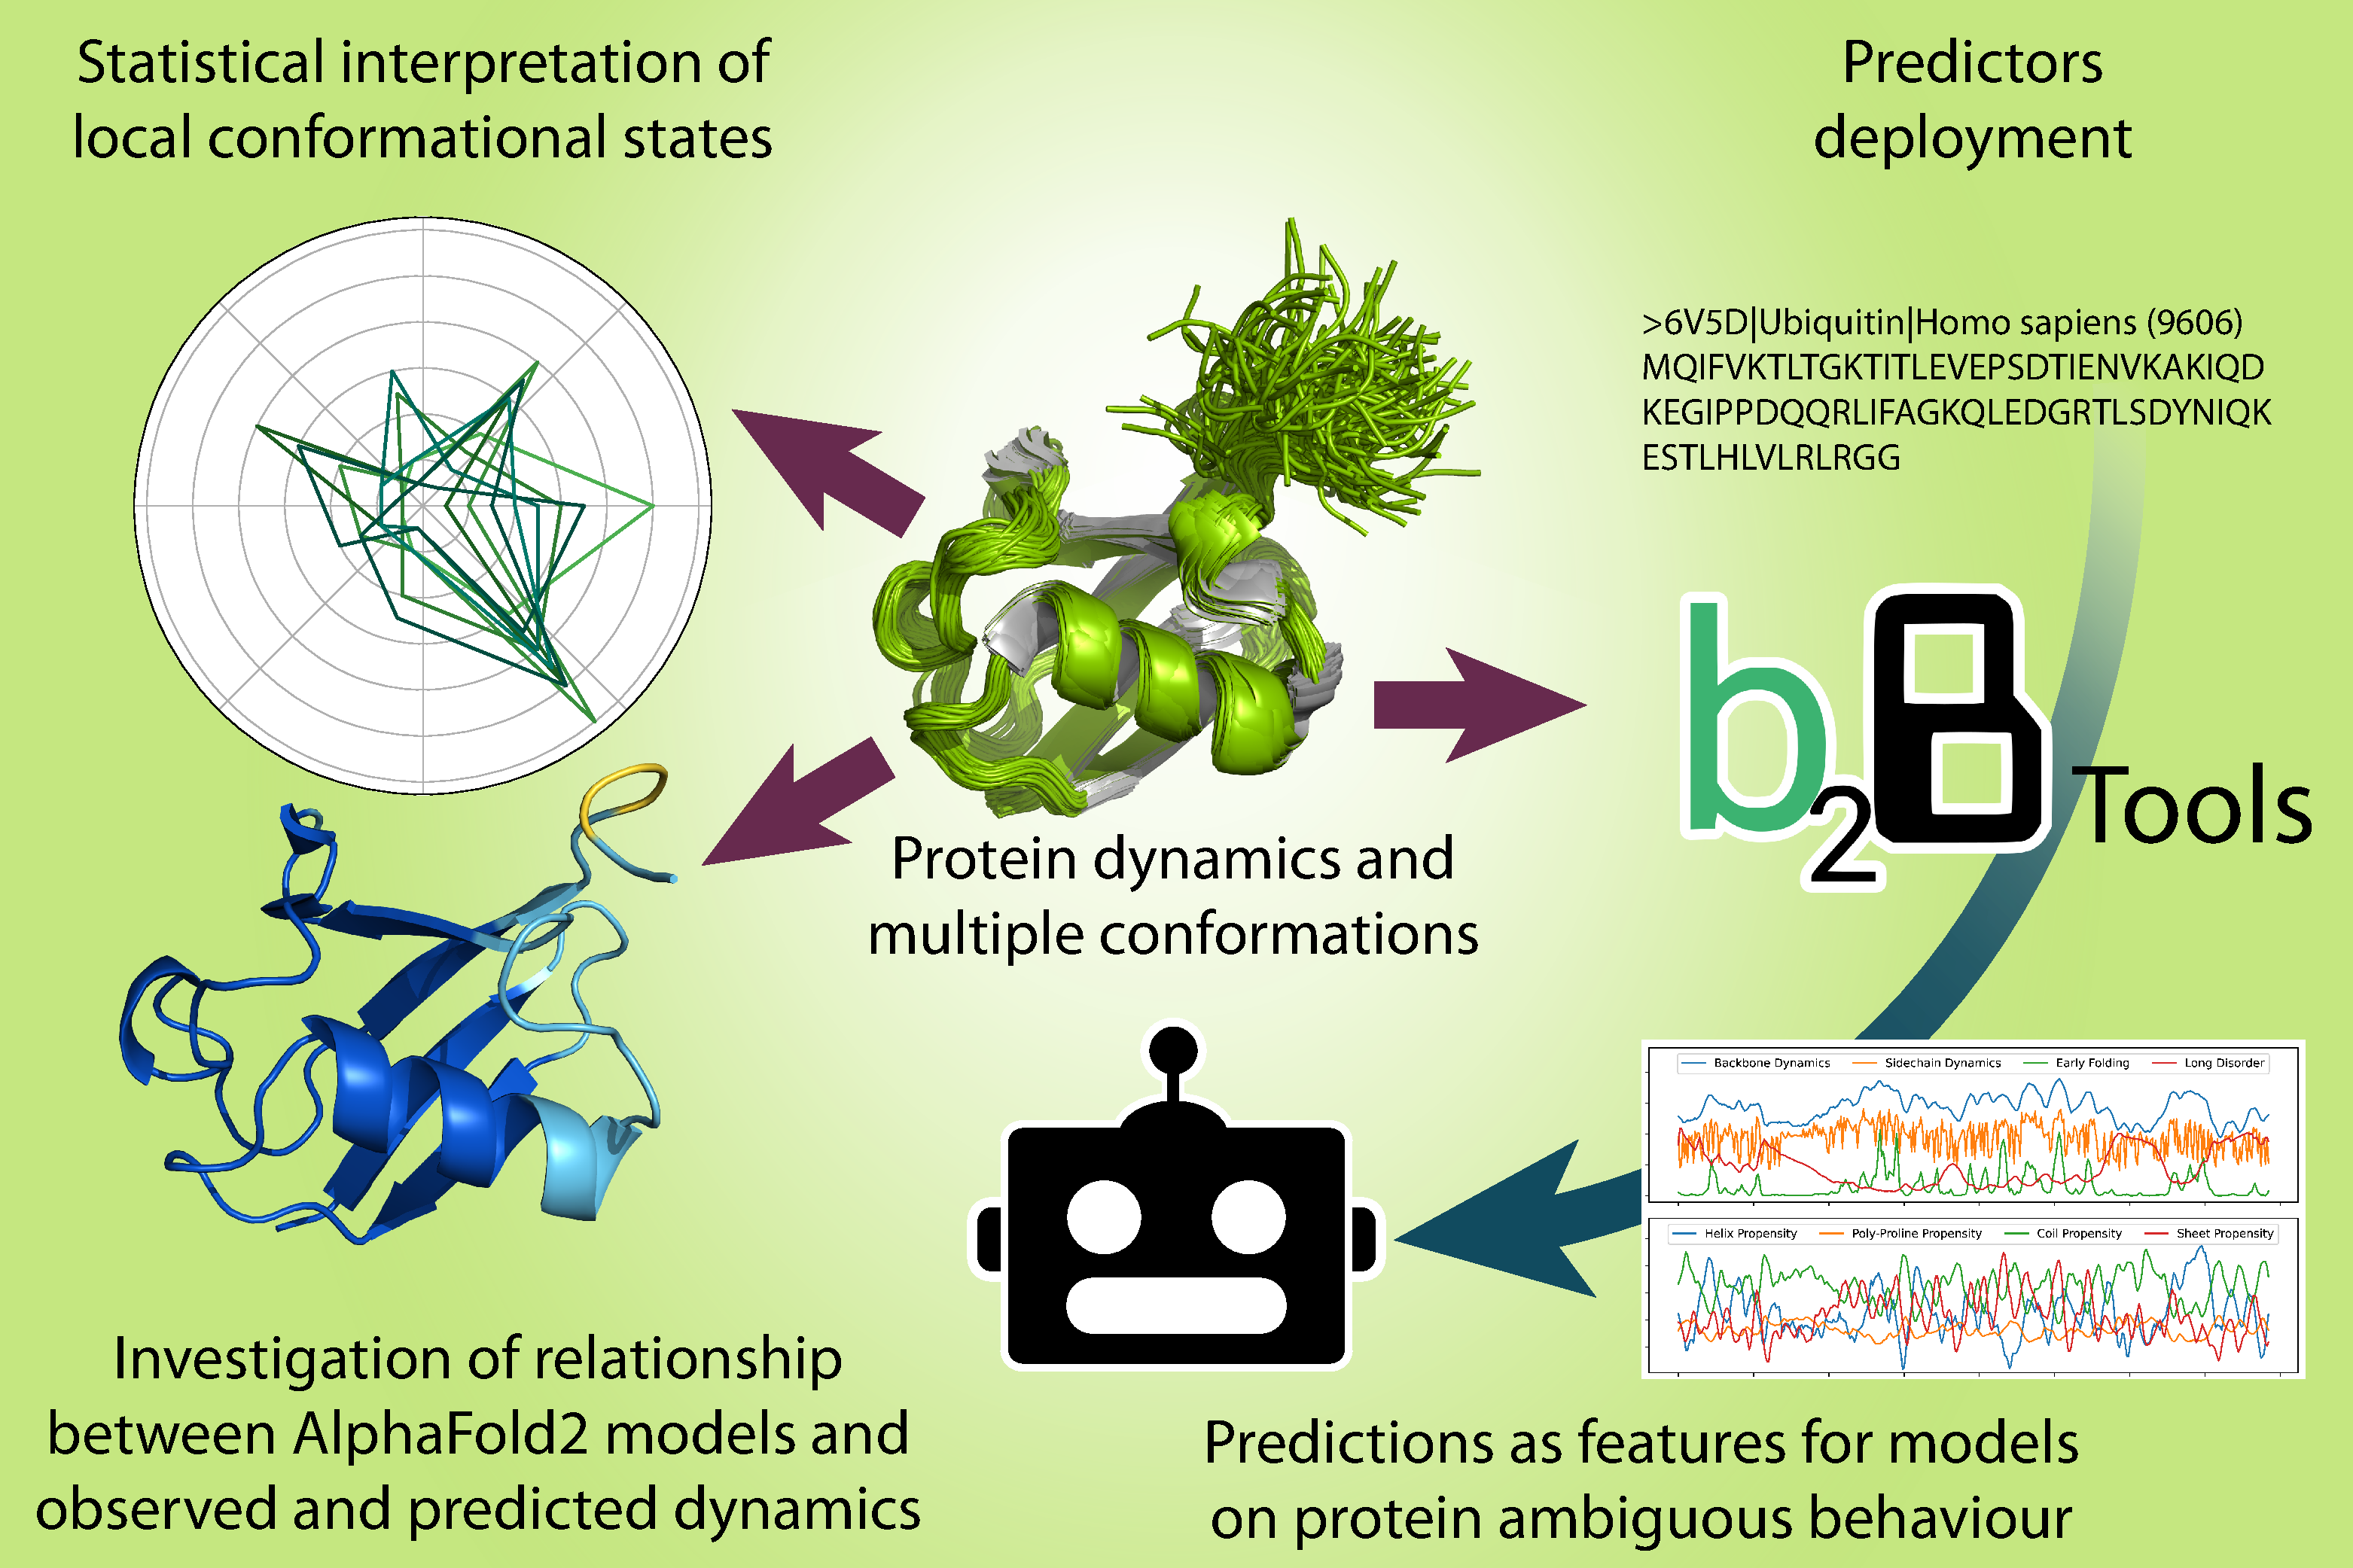
\includegraphics[width=\linewidth]{figures/overview_chapter2v2.pdf}
    \caption{\textbf{Overview of projects in this thesis.}
    This thesis keeps the dynamic nature of protein at its core, represented by the central NMR ensemble in this figure (PDB ID: 6V5D \cite{smith_enhancing_2020}). Chapter \ref{chapter:constava} introduces the novel method Constava, which produces residue-level probabilistic propensities of NMR-based conformational states as well as the capability of a residue to exist in multiple of them. Chapter \ref{chapter:b2btools_deployment} describes the path followed to unify the deployment of some of bio2Byte's most popular predictors into a single software suite: b2BTools. In chapter \ref{chapter:ambiguous}, the predictions from these tools are employed as features for a model to produce a residue-level biophysical interpretation order, disorder and ambiguity. Finally, chapter \ref{chapter:plddt} shows the relationship between AlphaFold2's pLDDT and protein dynamics, highlighting some novel nuances in their relationship (AlphaFold2 structure downloded from \burl{https://alphafold.ebi.ac.uk/entry/P0CG48}) 
    }
    \label{fig:chapter2:overview}
\end{figure}

The SARS-CoV-2 pandemic made the scientific community as a whole evaluate how they could contribute in the fight against the virus. In a team effort, the bio2Byte group employed our set of developed tools to estimate the biophysical properties of the virus' proteome. We also estimated these properties for each homologous protein and aligned them in a Multiple Sequence Alignment (\gls{msa}). The aligned predictions showed a biophysically-allowed space for each region, with narrower ranges indicating highly conserved properties and therefore potential targets to disrupt the normal function of a protein. These predictions were made publicly available in a web resource for its immediate availability and later published, now available in this thesis as part of chapter \ref{chapter:b2btools_deployment}. For this publication, I participated in selecting homologous proteins, creating \gls{msa}, and generating and formatting of the predictions, in addition to writing the corresponding section of the manuscript and testing the web resource.  

This effort made us realise that our tools were not as easy to deploy as a whole as we thought at the time. We then started working on the update of our tools, standardization of outputs, and their integration under a single suite: bio2Byte Tools. This suite was first offered as a web service (b2BTools server), which allowed execution either via user interface of Application Programmatic Interface (\gls{api}). This resource allowed the display of all bio2Byte Tools-derived biophysical predictions of a protein in a single view. It also allowed the visualisation of biophysically-allowed space, calculated from predictions calculated from a \gls{msa}. For this work, I directly contributed to the update of the tools.

We then decided to upgrade the deployment of our tools to match higher, more modern standards, and transformed bio2Byte Tools into a Python package. This firstly required the update of all tool's code, models, and dependencies. Then, the execution of the tools was interfaced in a wrapper object, which allowed simpler and unified execution of all tools. The Python package enables both direct interoperability of the obtained results or its storage in \textit{JSON}, \textit{CSV} or \textit{TSV} formats. With every update of the package, the results and execution are now thoroughly tested to ensure no deviation beyond floating point errors occur. The package is subsequently deployed in a variety of channels for both programmatic and non-programmatic usage, namely PyPI \cite{pypi}, Bioconda \cite{gruning_bioconda_2018}, Biocontainers \cite{da_veiga_leprevost_biocontainers_2017}, Galaxy Europe \cite{afgan_galaxy_2018} and in a set of in-house built Docker images (\href{https://hub.docker.com/r/bio2byte/b2btools}{https://hub.docker.com/r/bio2byte/b2btools}). This process is described in further detail in chapter \ref{chapter:b2btools_deployment} \cite{gavalda-garcia_bio2byte_2024}. 

Our work transformed this suite from being a collection of individual tools, with their own dependencies and environments, to being a single unified package, compliant with the FAIR principles. This now allows our suite to be \textit{\Glspl{findability}} and \textit{\Glspl{accessibility}} in different deployment channels \cite{pypi, gruning_bioconda_2018}, archived in Biocontainers \cite{da_veiga_leprevost_biocontainers_2017}, and interfaced on Galaxy Europe \cite{afgan_galaxy_2018} for non-programmatic usage. It also features an \textit{\Glspl{interoperability}} output in standardised formats. Finally, bio2Byte Tools is \textit{\Glspl{reusability}} beyond any dependency, with the creation of Docker containers, insensitive to any future dependency changes. For this work, I developed, implemented and validated the software suite and Continuous Integration and Continuous Deployment (\gls{cicd}) pipelines in close collaboration with Adrian Díaz, and lead the writing of the manuscript (Chapter \ref{chapter:b2btools_deployment}) \cite{gavalda-garcia_bio2byte_2024} and creation of figures. 

Before the final deployment of bio2Byte tools, an earlier version of the tools was employed as part of an assessment to describe proteins with ambiguous behaviour (chapter \ref{chapter:ambiguous}) \cite{roca-martinez_challenges_2022}. My contribution to this analysis is featured in the analysis of AlphaFold2's \gls{plddt} metric for local predictive confidence in relation to bio2Byte's estimations of protein biophysics. The relation between predicted metrics and \gls{plddt} indicated a relationship between highly dynamic regions and and low AlphaFold2 predictive confidence. This relation was shown more clearly when the residues were stratified according to curated order preferences, available in the generated datasets for this work \cite{roca-martinez_challenges_2022}. This work showed the need for a more in-depth analysis of the relationship between \gls{plddt} and protein biophysics, with focus on experimental metrics of protein \gls{dynamics} and \gls{flexibility}. 

In chapter \ref{chapter:plddt} \cite{gavalda-garcia_gradations_2024}, we show a large-scale analysis of AlphaFold2's models in relation to \gls{nmr}-derived \glspl{conformationalensemble} and metrics and diverse computational descriptions of \gls{dynamics} and conformational heterogeneity. For this analysis, I performed the work in relation to metrics derived from \gls{nmr} and Molecular Dynamics, data integration, creation of the code repository and its associated docker image to reproduce the analysis, and I equally contributed with Adrian Díaz to build the interactive analysis in the web server. Bhawna Dixit produced the entirety of the \glspl{nma} for the proteins' AlphaFold2 models and, when available, their \gls{nmr} \glspl{conformationalensemble}. We concluded that AlphaFold2's low \gls{plddt} values tend to co-occur with highly dynamic regions, and so the opposite was true with high \gls{plddt} values and low \gls{dynamics}. This metric, however, was unable to describe gradations in \gls{dynamics}. 

We could also observe that biases on the training set, derived from the removal of ligands from the protein structures, contributed to an overestimation of protein regions rigidity, illustrated by high \gls{plddt} contrasting with \gls{nmr}-assessed dynamic regions. The analysis also showed distinct \gls{plddt} distributions for residues which adopt different conformational states. Interestingly, residues in a relaxed Sheet conformational state (chapter \ref{chapter:constava} \cite{gavalda-garcia_data-driven_2024}) displayed higher \gls{plddt} than those in a stable Helix \gls{conformation}. We hypothesise that such difference originates in the stronger evolutionary signal required to predict Sheet \glspl{conformation} due to the long-range hydrogen bonds required to stabilise this secondary structure, and acquired in AlphaFold2 in its \gls{msa} modules. Helix \glspl{conformation}, on the other hand, are stabilised by near-local, periodic hydrogen bonds, which we argue that permits more \gls{flexibility} in its amino acid sequence and subsequently a weaker signal from the \gls{msa} modules. 

We also find that residues with diverse \glspl{conformation} in their \gls{nmr} \glspl{conformationalensemble} follow lower \gls{plddt} distributions than their unique \gls{conformation} counterparts (Chapter \ref{chapter:plddt}, Supplementary Fig. 5.10). This difference is further accentuated when the secondary structure between \gls{nmr} \glspl{conformationalensemble} and AlphaFold2 models mismatches (Chapter \ref{chapter:plddt}, Supplementary Fig. 5.11). We observe a notable behaviour in residues with an \gls{nmr}-derived consensus \gls{alphahelix} or \gls{betasheet} assignment: i) The match in consensus \gls{nmr} and AlphaFold2 secondary structure assignments for residues without a unique \gls{nmr} assignment results in higher \gls{plddt} distributions than for ii) those with a unique \gls{nmr} assignment which mismatches with AlphaFold2's assignment (Supplementary Fig 5.11, A \& J). 

Residues with a high propensity to acquire a secondary structure, but able to exist in other \glspl{conformation}, will potentially be present in AlphaFold2's training set only in their rigid \gls{conformation}, therefore resulting in high \glspl{plddt}. This is due to the further stabilisation of these structures in the experimental conditions for \gls{xraycrystallography} crystallography or \gls{cryoem}. The existence of Helix and Sheet residues with unique \gls{nmr} assignments which mismatch AlphaFold2's assignments are most likely explained by \gls{folduponbinding} regions, stabilised in the training data set by their ligands, which are then removed. 

This \gls{folduponbinding} is further suggested by the homologous distributions for \gls{nmr}-assigned Coil and Turn residues, which feature higher \gls{plddt} values for residues with unique \gls{nmr} assignments that mismatch with AlphaFold2 than for residues with non-unique \gls{nmr} assignments with matching AlphaFold2 assignment (Supplementary Fig 5.11, D \& G). This indicates higher predictive confidence in residues which acquire a defined, stable structure upon binding over residues which can exist in multiple \glspl{conformation} in their unbound state. Overall, this analysis indicated that the inclusion of only static structures and the removal of binding from AlphaFold2's training set results in difficulties in the assessment of regions that can adopt multiple \glspl{conformation} or fold upon binding. 

Keeping in mind the challenge in representing protein \gls{conformation} from a dynamic perspective, we developed Constava (Chapter \ref{chapter:constava}), a method to measure the capacity of protein residues to exist in multiple conformational states, and how often it transitions among them \cite{gavalda-garcia_data-driven_2024}. This is the result of a close collaboration with Dr. David Bickel to develop, validate and understand the data-driven, probabilistic definition of conformational states propensities and conformational state variability. To achieve this, six conformational states (\textit{Core Helix}, \textit{Surrounding Helix}, \textit{Coil}, \textit{Turn}, \textit{Surrounding Sheet}, and \textit{Core Sheet}) were defined as \glspl{pdf}s in the backbone dihedral space. ShiftCrypt-interpreted \gls{nmr} chemical shifts \cite{orlando_shiftcrypt_2020} values were employed, in combination with STRIDE \cite{frishman_knowledge-based_1995} secondary structure assignments of all models in our experimental \gls{nmr} data set, to identify suitable amino acids to train each of the six \glspl{pdf}s. These conformational states reflect the dynamism of protein structures better than methods designed to be applied to static structures.


Constava leverages information from a collection of static structures, such as \gls{md} trajectories, to derive a continuous probabilistic description of local \textcolor{red}{backbone} \gls{dynamics}, in the form of conformational state variability, and conformational preferences, as conformational state propensities. A sliding window approach is recommended for time-series data, such as \gls{md} trajectories, but bootstrapping is also allowed over a ensemble of structures with no relation between adjacent elements, which enables its usage on \gls{nmr} \glspl{conformationalensemble}. Our results also show that Constava can detect a region's propensity to adopt a certain \gls{conformation} before it fully emerges in an \gls{md} simulation. This has potential applications in \gls{md} simulations, informing about a potentially insufficient sampling of a protein's \gls{conformation}, It can also be applied to protein design, as it can detect regions that could adopt a certain \gls{conformation} if a neighbouring amino acid is substituted to boost that dormant propensity. Overall, Constava offers a new set of metrics to probabilistically describe a protein as the biophysically allowed range of \glspl{conformation} in which it can exist.
